% 温故错题本 iOS

%% UTF-8

\documentclass[UTF8,a4paper,openany]{ctexart}
\usepackage{color}
\usepackage{graphicx}
\usepackage[colorlinks,linkcolor=red,anchorcolor=blue,citecolor=green]{hyperref}
\usepackage{float}
\usepackage{bbding}


\title{温故错题本(iOS) \\v1.01}
\author{盐城欧布科技有限公司}
\date{\today}

\hypersetup{
	pdftitle={温故错题本(iOS) },
	pdfauthor={盐城欧布科技有限公司}
}

\begin{document}
	\maketitle
	\tableofcontents
	\section{简介}

\begin{figure}[H]
\centering

\includegraphics{img/logo.jpg}
\end{figure}
温故而知新。作业、考试、课外习题等不断产生错题,如何整理错题本?手抄,慢,花费时间长,很难坚持下去。剪贴,乱,可能需要额外复印空白题目。

你需要一个可以快速整理错题(拍照→剪切→涂改→保存),随时可以回顾复习的错题本app。\\

官网:\url{http://www.ycorb.com/}\\

此帮助适用于苹果iOS系统。


\section{开始}
\subsection{打开}
\begin{figure}[H]
	\centering
	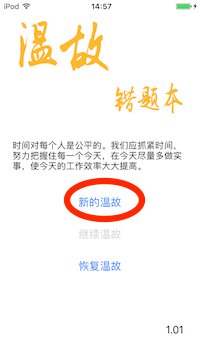
\includegraphics{img/1.png}
	\caption{首次打开}
	\label{img1}
\end{figure}
首次打开app,界面如图(\ref{img1})所示。点击“新的温故”进入数据初始化。

“恢复温故”使用请见后面\ref{restore}节。

数据初始化成功后,进入app初始默认页面,如图(\ref{img4})。
\begin{figure}[H]
	\centering
	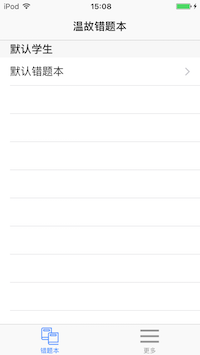
\includegraphics{img/4.png}
	\caption{默认页面}
	\label{img4}
\end{figure}

可以看到有一个默认学生,他有一本默认错题本。

\section{使用}
\subsection{学生管理}
支持多学生管理。低年级学生通常由家长帮助一起整理错题本,家里有多个孩子时适用。

点击底部“更多”菜单,如图(\ref{img5}),打开,如图(\ref{img6})。
\begin{figure}[H]
	\centering
	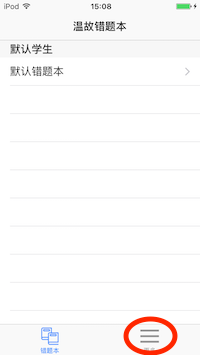
\includegraphics{img/5.png}
	\caption{更多菜单}
	\label{img5}
\end{figure}

\begin{figure}[H]
	\centering
	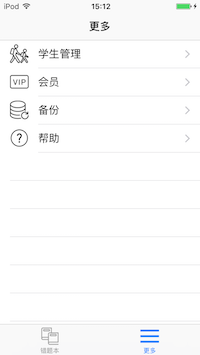
\includegraphics{img/6.png}
	\caption{菜单}
	\label{img6}
\end{figure}

点击“学生管理”,进入学生列表,如图(\ref{img7})。

\begin{figure}[H]
	\centering
	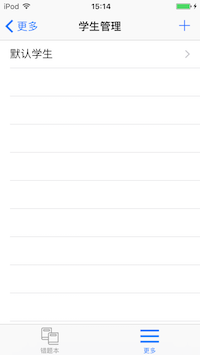
\includegraphics{img/7.png}
	\caption{学生列表}
	\label{img7}
\end{figure}

\subsubsection{增加学生}
我们这里新增加一个学生叫“小明”,点击右上角加号图标,如图(\ref{img8})。
\begin{figure}[H]
	\centering
	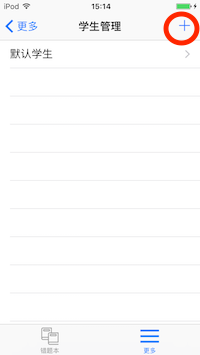
\includegraphics{img/8.png}
	\caption{+号图标}
	\label{img8}
\end{figure}

在文本框中输入“小明”,点击“增加”,如图(\ref{img9})
\begin{figure}[H]
	\centering
	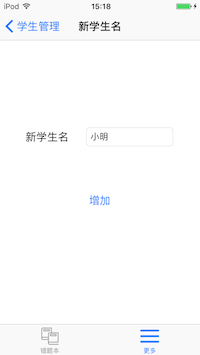
\includegraphics{img/9.png}
	\caption{增加学生}
	\label{img9}
\end{figure}

增加成功后,页面再次跳转到学生列表,如图(\ref{img10}),我们可以看到“小明”

\begin{figure}[H]
	\centering
	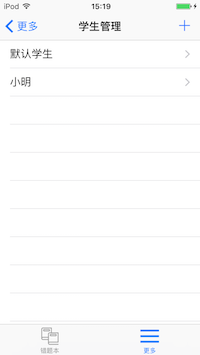
\includegraphics{img/10.png}
	\caption{学生列表}
	\label{img10}
\end{figure}

\subsubsection{修改学生名}
修改“默认学生”到“小红”,点击“默认学生”,进入错题本管理,如图(\ref{img11})。
\begin{figure}[H]
	\centering
	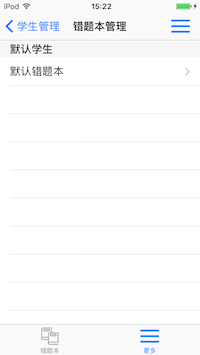
\includegraphics{img/11.png}
	\caption{进入}
	\label{img11}
\end{figure}

点击右上角菜单,选择”修改学生“,进入修改页面,修改文本框中的“默认学生”到“小红”,点击修改按钮,如图(\ref{img12})。
\begin{figure}[H]
	\centering
	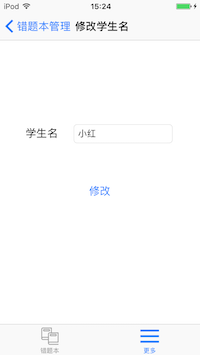
\includegraphics{img/12.png}
	\caption{修改到小红}
	\label{img12}
\end{figure}

修改成功后,页面回到”错题本管理“,点击左上角”学生管理“,回到学生列表,可以看到“默认学生”变成了“小红”,如图(\ref{img13})。
\begin{figure}[H]
	\centering
	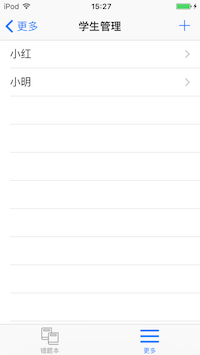
\includegraphics{img/13.png}
	\caption{学生列表}
	\label{img13}
\end{figure}

\subsubsection{删除学生}
\label{delete_student}
在”错题本管理“页面,点击右上角菜单,选择”删除学生“如图(\ref{img14})。
\begin{figure}[H]
	\centering
	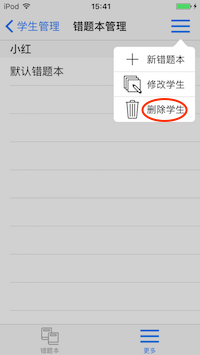
\includegraphics{img/14.png}
	\caption{删除学生}
	\label{img14}
\end{figure}

在菜单中,选择“删除”。注意:当此学生下面没有错题本时,才可删除。

\subsection{错题本管理}
\subsubsection{增加错题本}
我们现在给小红增加一个错题本“一年级数学(下)”。在学生管理--学生列表中找到小红,点击进入错题本管理,如图(\ref{img15}),可以看到,小红已经有一个“默认错题本”。
\begin{figure}[H]
	\centering
	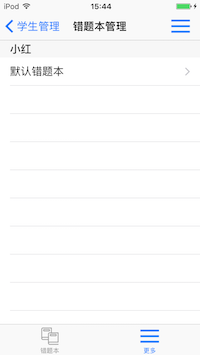
\includegraphics{img/15.png}
	\caption{错题本列表1}
	\label{img15}
\end{figure}

点击右上角菜单,选择”新错题本“,进入新错题本增加页面,完成增加后如图(\ref{img16})。
\begin{figure}[H]
	\centering
	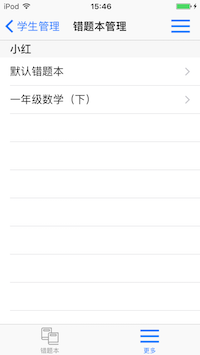
\includegraphics{img/16.png}
	\caption{错题本列表2}
	\label{img16}
\end{figure}

\subsubsection{修改错题本}
修改小红的“默认错题本”到“一年级语文(下)”,在图(\ref{img16})中,点击“默认错题本”,进入修改错题本页面。修改完成后如图(\ref{img17})。
\begin{figure}[H]
	\centering
	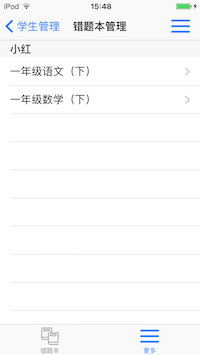
\includegraphics{img/17.png}
	\caption{错题本列表3}
	\label{img17}
\end{figure}

\subsubsection{删除错题本}
类似删除学生(\ref{delete_student}),也是在”修改错题本“页面,点击右上角菜单。注意:当此错题本下所有错题全部复习完成,才可删除。
	\subsection{错题本}
现在的主界面如图(\ref{img18})
\begin{figure}[H]
	\centering
	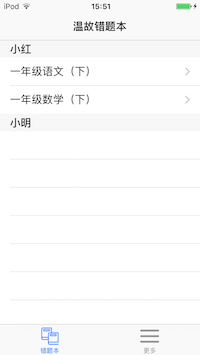
\includegraphics{img/18.png}
	\caption{主界面}
	\label{img18}
\end{figure}
现在在小红的错题本“一年级数学(下)”里面添加错题,点击“一年级数学(下)”条目进入错题本,如图(\ref{img19})
\begin{figure}[H]
	\centering
	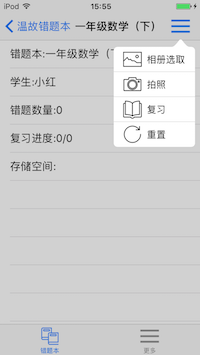
\includegraphics{img/19.png}
	\caption{一年级数学(下)}
	\label{img19}
\end{figure}
此页面显示了错题本名、学生名、错题数量、复习进度(已经复习/错题数量)、存储空间。

右上角是几个操作按钮、分别是复习、相册选取、拍照、重置。

\subsubsection{增加错题}
步骤1:可以选择“相册选取”或“拍照”获得一张错题照片。建议手机横拍。这里需要权限(拍摄照片、存储等),请允许。
\begin{itemize}
	\item 相册选取(建议,效率更高。先集中一起拍照,然后从相册中一张张选择处理)
	\item 拍照(拍一张,处理一张)
\end{itemize}

步骤2:把照片裁剪到合适的大小,如图(\ref{img20})。满意点击右上角\Checkmark ,进入裁剪。不满意,点击左上角\XSolid ,退回错题本。

\begin{figure}[H]
	\centering
	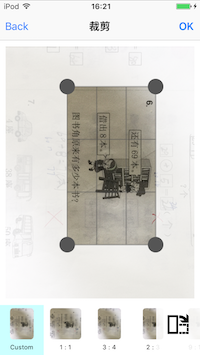
\includegraphics{img/20.png}
	\caption{裁剪}
	\label{img20}
\end{figure}

步骤3:涂改掉多余的答案等,仅保留题干,如图(\ref{img21})。左上角回退菜单会退回到错题本。右上角第一个是撤销一次涂改,第二个是进入步骤4。
\begin{figure}[H]
	\centering
	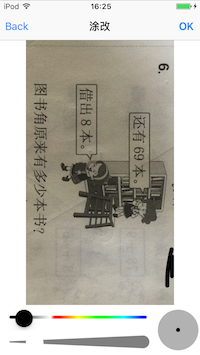
\includegraphics{img/21.png}
	\caption{涂改}
	\label{img21}
\end{figure}

步骤4:如图(\ref{img22}),就是复习是会看到的错题。可选操作,右上角有3个按钮,分别是错解、正解、总结,可以为这道错题添加上错误的解法、正确的解法、自己的归纳总结等(还是通过“拍照→剪切→涂改→保存”这个步骤录入。)。如果不需要额外增加信息,可以直接点击左上角回退到错题本。
\begin{figure}[H]
	\centering
	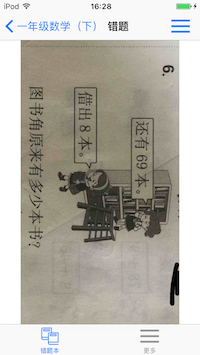
\includegraphics{img/22.png}
	\caption{错题浏览}
	\label{img22}
\end{figure}

现在的错题本看上去是这样,如图(\ref{img23})
\begin{figure}[H]
	\centering
	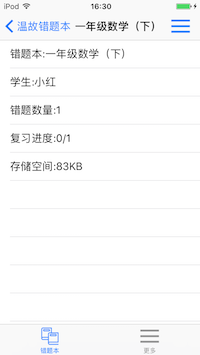
\includegraphics{img/23.png}
	\caption{错题本}
	\label{img23}
\end{figure}

\subsection{复习}
\begin{figure}[H]
	\centering
	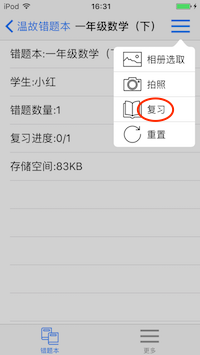
\includegraphics{img/24.png}
	\caption{进入复习}
	\label{img24}
\end{figure}

点击“复习”菜单,如图(\ref{img24}),进入复习页面,如图(\ref{img25})。这里是随机复习模式,低年级学生在家长陪同的情况下使用,因为需要随时批改。不能随时批改的情况下,建议使用“测验模式”。

\begin{figure}[H]
	\centering
	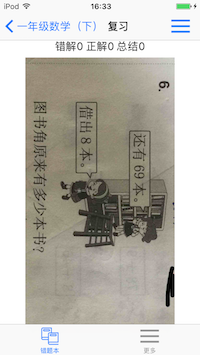
\includegraphics{img/25.png}
	\caption{复习}
	\label{img25}
\end{figure}

随机从未复习的错题中选择一题,根据本次答题情况,分别选择\Checkmark 或 \XSolid 按钮。回答正确的,本轮复习中不会再次出现。

右上角下拉菜单中,有错解、正解、总结按钮,可以这时增加当前错题的错解、正解、总结。移动按钮可以移动当前错题到其他错题本中。删除按钮,可以删除当前错题。

\subsection{测验}
批量复习,批量批改。
\begin{figure}[H]
	\centering
	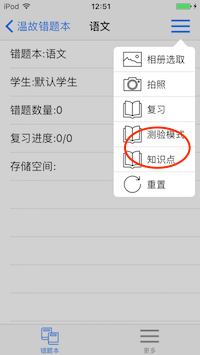
\includegraphics{img/32.png}
	\caption{进入测验}
	\label{img32}
\end{figure}
点击“测验模式”菜单进入测验列表,如图(\ref{img32})

点击右上角“+”,选择本次测验的题目数量,增加新测验,如图(\ref{img33})。
\begin{figure}[H]
	\centering
	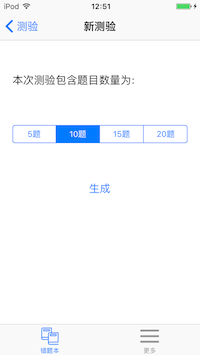
\includegraphics{img/33.png}
	\caption{新测验}
	\label{img33}
\end{figure}

从测验列表(\ref{img34})进入测验复习
\begin{figure}[H]
	\centering
	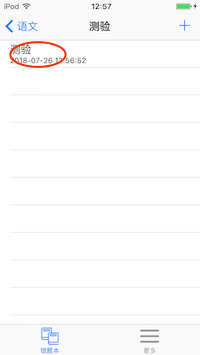
\includegraphics{img/34.png}
	\caption{测验列表}
	\label{img34}
\end{figure}

学生通过右上角上下箭头,切换题目,(\ref{img35})
\begin{figure}[H]
	\centering
	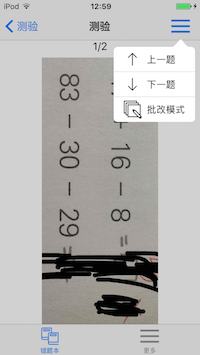
\includegraphics{img/35.png}
	\caption{测验}
	\label{img35}
\end{figure}

家长可以通过右上角菜单“批改模式”,进入批改状态,如图(\ref{img36})
\begin{figure}[H]
	\centering
	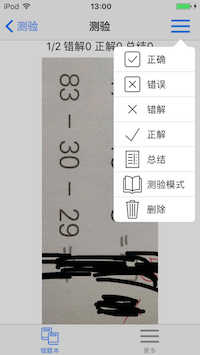
\includegraphics{img/36.png}
	\caption{测验批改}
	\label{img36}
\end{figure}
根据本次答题情况,分别选择\Checkmark 或 \XSolid 按钮。回答正确的,本轮复习中不会再次出现。可以这时增加当前错题的错解、正解、总结。删除是删除当前测验。

\subsection{知识点}
进入知识点列表,如图(\ref{img37})
\begin{figure}[H]
	\centering
	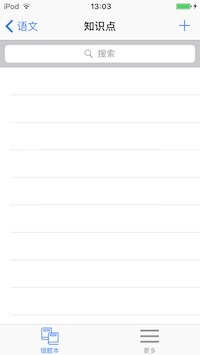
\includegraphics{img/37.png}
	\caption{知识点列表}
	\label{img37}
\end{figure}
点击右上角“+”,进入增加页面,如图(\ref{img38})。放大镜图标,可以按标题搜索。
\begin{figure}[H]
	\centering
	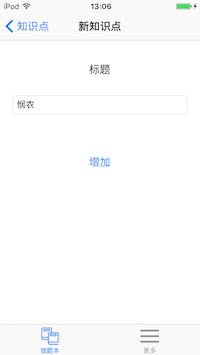
\includegraphics{img/38.png}
	\caption{增加知识点}
	\label{img38}
\end{figure}
在知识点列表中,点击刚刚增加的“春晓”,进入知识点页面,如图(\ref{img39})
\begin{figure}[H]
	\centering
	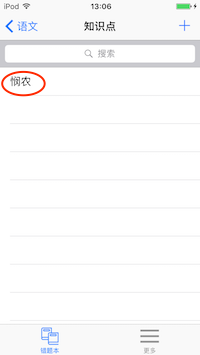
\includegraphics{img/39.png}
	\caption{知识点}
	\label{img39}
\end{figure}
现在可以通过拍照、相册选取,加入多张知识点图片,如图(\ref{img40})
\begin{figure}[H]
	\centering
	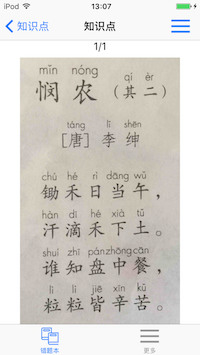
\includegraphics{img/40.png}
	\caption{知识点}
	\label{img40}
\end{figure}
上下箭头,可以在多张图片中切换。删除可以删除一张图片。删除知识点可以删除当前知识点。

\subsection{重置}
\begin{figure}[H]
	\centering
	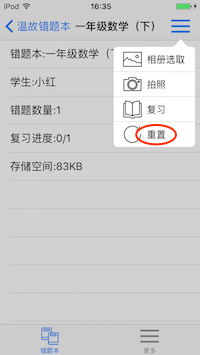
\includegraphics{img/26.png}
	\caption{重置}
	\label{img26}
\end{figure}
错题本中的错题全部复习完成,点击如图(\ref{img26})按钮可以重新重置错题状态为可复习状态。
	\section{会员}

\subsection{登录}
\begin{figure}[H]
	\centering
	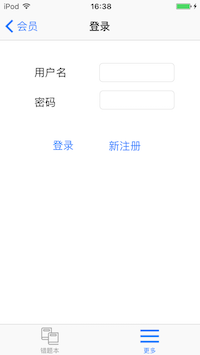
\includegraphics{img/27.png}
	\caption{登录}
	\label{img27}
\end{figure}
如图(\ref{img27}),输入用户名和密码登录。如果还没有用户名和密码,点击“新注册”。

本公司产品通用一套用户名和密码。如果注册过,直接用以前的用户名和密码登录即可。

\subsection{注册}
\begin{figure}[H]
	\centering
	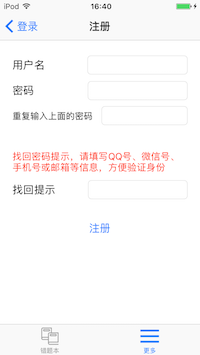
\includegraphics{img/28.png}
	\caption{注册}
	\label{img28}
\end{figure}
如图(\ref{img28}),输入用户名、密码、找回密码提示等信息,点击“注册”。

注意:2次密码输入要一致。找回密码提示需要填写QQ号、微信号、手机号码、邮箱,客服依据填写信息确定用户是否是本人后,提供服务。

本公司产品通用一套用户名和密码。如果提示用户名已经被使用,请确认是否在本公司其他产品中注册过。如果注册过,直接用以前的用户名和密码登录即可。

\subsection{升级会员}
\begin{figure}[H]
	\centering
	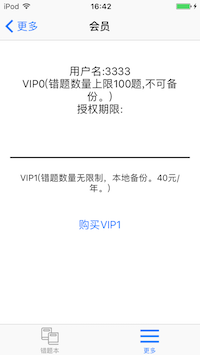
\includegraphics{img/29.png}
	\caption{升级会员}
	\label{img29}
\end{figure}
如图(\ref{img29}),可以直接升级会员。付费后,退出当前页面,重新进入。

\begin{itemize}
	\item VIP0,默认,错题数量上限100题,不可本地备份。
	\item VIP1,错题数量无限制,可本地备份。可注册登录后购买,30元/年,限本人使用。
\end{itemize}

\section{分享}
\begin{figure}[H]
	\centering
	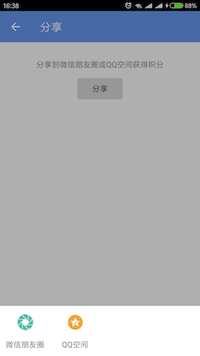
\includegraphics{img/30.png}
	\caption{分享}
	\label{img30}
\end{figure}
如图(\ref{img30}),可分享到微信朋友圈、QQ空间。每次成功分享后,分享积分+1
\begin{itemize}
	\item 分享积分累计7分后,可以免费备份1次。备份后,累计分-7分。
	\item 当日分享后,可以无限制添加错题。
\end{itemize}

\section{备份}
\begin{figure}[H]
	\centering
	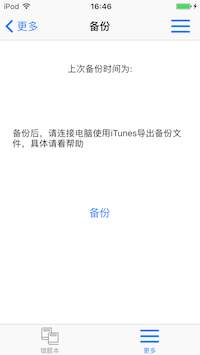
\includegraphics{img/31.png}
	\caption{备份}
	\label{img31}
\end{figure}
如图(\ref{img31}),积累的错题,是珍贵的学习资料,不容有失。

VIP1会员或分享积分7分以上,可以进行备份。

备份到SD卡根目录(如果有安装)或内部存储根目录的wgctb目录下。

备份文件,不受app卸载影响。但是任然仅保存在手机中,强烈建议备份后,再次备份到电脑、网盘(比如微云、百度网盘)等。可以在文件管理中搜索wgctb,找到备份文件。\newline

右上角菜单
\begin{itemize}
	\item 整理数据(删除错题、错题本后,备份文件大小不见减少时,可以使用整理数据功能,压缩备份文件大小)
	\item 清理备份(删除wgctb备份目录下的所有备份文件,建议在备份文件已经再次备份到电脑或云盘后使用)
\end{itemize}

\section{恢复备份}
\label{restore}
\begin{figure}[H]
	\centering
	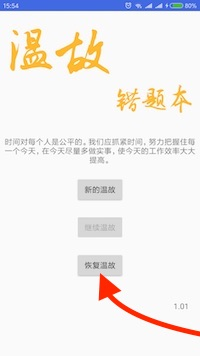
\includegraphics{img/2.jpg}
	\caption{进入恢复}
	\label{img2}
\end{figure}

重新安装app后,可以选择“恢复温故”,如图(\ref{img2}),进入恢复备份页面,如图(\ref{img3})

\begin{figure}[H]
	\centering
	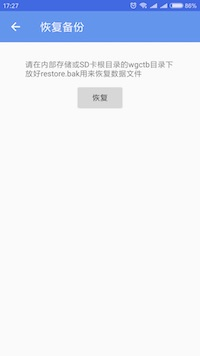
\includegraphics{img/3.jpg}
	\caption{恢复}
	\label{img3}
\end{figure}

选择一个历史备份,重命名为restore.bak,放置于内部存储或SD卡根目录的wgctb目录下,点击“恢复”,让错题本数据恢复到备份时的状态。如果提示需要访问存储权限,请允许。

\section{升级}
升级app,请使用覆盖更新方式,直接安装新的app版本。千万不要先删除,后安装,这样会丢失所有错题数据。
\end{document}
